\section{Differential geometry}

\label{section: differential geometry}

\todo[inline]{Integrate old and new notes, fix citations}






\subsection{Old Notes}


\subsubsection*{Topology} 
Based on Carroll and
% \footnote{
%     \url{https://en.wikipedia.org/wiki/Topological_space}, 
%     \url{https://en.wikipedia.org/wiki/Homeomorphism}, and 
%     \url{https://en.wikipedia.org/wiki/Continuous_function#Continuous_functions_between_topological_spaces}
%     }.
In general relativity, space-time is modeled as a \emph{differentiable manifold} $\mathcal{M}$.
A differentiable manifold is a mathematical space which we may draw coordinates on, enabling us to do calculus.
It generalizes the familiar notion of euclidean space. 
Manifolds are a special kind of topological space, so this is the first structure we need to define.

A topological space is a set of points $p \in S$, as well as a topology $\mathcal{T}$.
The topology contains \emph{open sets} of $S$.
Both $S$ itself, and the empty set $\emptyset = \{\}$ must be part of the topology $\mathcal{T}$.
Open sets must obey the rule that the union of two open sets again is an open set, i.e. $\{U_i\}_i \subseteq \mathcal{T}, \implies \cup_i U_i \in \mathcal{T}$.
All \emph{finite intersections} of open sets be open sets, i.e. $\{U_i\}_{i=1}^N \subseteq \mathcal{T}, \implies \cap_i U_i \in \mathcal{T}$. 
The structure of the topology allows one to talk about a neighborhood of a point $p \in S$, and define a homeomorphism. \footnote{Not to be confused with homomorphism.}
\begin{definition}
    A \emph{neighbourhood} of a point $p$ is a open set $U$ which contain $p$.    
\end{definition}
As $S$ is an open set, all points have a neighbourhood. to define homeomorphism, we need a notion of a continuous function. 
The definition of continuous coincide with the regular $\epsilon, \delta$ definition from calculus when the topological space in question is $\mathbb{R}$ and the topology is open line intervals.
However, the topology allows for a more general definition of continuous function:
\begin{definition}
    A function between two topological spaces $f: S \rightarrow T$ is \emph{continuous} if and only if, for every open set $V \subseteq T$, the pre-image $f^{-1}(V) = U \subseteq S$ is open.
\end{definition}
\begin{definition}
    A \emph{homeomorphism} $f: S \rightarrow T$ is then a continuous, bijective function whose inverse $f^{-1}$ also is continuous. 
\end{definition}



\subsubsection*{Manifolds and tensors}



A manifold $\mathcal{M}$ is a topological space with additional structure. All points $p \in S$ are locally \emph{homeomorphic} to euclidian space $\mathbb{R}^n$. A open set $U \in \mathcal{T}$ and a corresponding homeomorphism
\begin{equation*}
    x: \, U \longrightarrow \mathbb{R}^n,
\end{equation*}
called a coordinate function, together form a chart $(x, U)$.
This chart takes points $p \in U$ and gives them coordinates $x(p) = (x_1(p), \dots x_n(p)) \in \mathbb{R}^n$.
A set $\mathcal{A} = \{(x^i, U_i)\}$ such that $\{U_i\}$ cover $S$ is an atlas.
A manifold $\mathcal{M}$ is thus a topological space together with the maximal atlas, i.e. the larges possible atlas.
To get a differentiable manifold, we demand that the transition functions
\begin{equation*}
    \tau^{i,j} = x^j \circ (x^i)^{-1}: \, x^i(U_i \cap U_j) \longrightarrow x^j(U_i \cap U_j)
\end{equation*}
of the atlas are infinitely differentiable, or smooth.

Let $\gamma: \mathbb{R} \rightarrow \mathcal{M}$ be a curve in the manifold.
This may be used to define a directional derivative of functions $f:\, \mathcal{M} \rightarrow \mathbb{R}$ on the manifold. 
Let $\lambda$ be the parameter associated with $\gamma$. 
The derivative is then
\begin{equation*}
    \odv{f}{\lambda} = \odv{\lambda} (f\circ\gamma)(\lambda).
\end{equation*}
For a given point $p \in \mathcal{M}$, and form an equivalence class of curves $[\gamma]_p$ that gives the same directional derivative at $p$.\footnote{Called a germ} The set of all such derivative operators form a vector space, the tangent space
\begin{equation*}
    T_p = \left\{ { \odv{}{\lambda} (\_ \circ\gamma)(\lambda_0) \,\Big| \, [\gamma]_p(\lambda_0) = p }\right\}.
\end{equation*}
Using the chain rule, the coordinate functions $x^\mu$ induce a basis for the tangent space:
\begin{equation*}
    \odv{f(\gamma(\lambda))}{\lambda} = \odv{}{\lambda}[(f \circ x^{-1})(x \circ \gamma)](\lambda) 
    = \pdv{x^\mu}(f \circ x^{-1}) \odv{}{\lambda}(x \circ \gamma)^\mu = \odv{x^\mu}{\lambda}\partial_\mu f.
\end{equation*}
Thus, $V^\mu = \odv{x^\mu}{\lambda}$ are the components of the vector, and $e_\mu = \partial_\mu$ the basis. If we change coordinates on the manifold, $x \rightarrow x'$, we get a transition function $\tau = x \circ (x')^{-1}$.
This coordinate change induces a basis change in the tangent space, yielding new basis vectors
\begin{equation*}
    \partial_\mu' = \pdv{}{x'^\mu} = \pdv{\tau^\nu(x')}{x'^\mu} \pdv{}{x^\nu} = \pdv{}{x^\nu}{x'^\mu} \partial_\nu.
\end{equation*}
This again induces a change of the components,
\begin{equation*}
    V'^\mu = \pdv{x'^\mu}{x^\nu} V^\nu, 
\end{equation*}
ensuring that
\begin{equation*}
    V'^\mu e'_\mu = V^\nu \pdv{x'^\mu}{x^\nu} \pdv{x^\rho}{x'^\mu} \partial_\rho = V^\mu e_\mu.
\end{equation*}
We saw that a function $f: \, \mathcal{M} \rightarrow \mathbb{R}$ has, at $p \in \mathcal{M}$, the directional derivative
\begin{equation*}
    \odv{f}{\lambda} \bigg |_{\lambda_0} = V^\mu \pdv{f}{x^\mu}
\end{equation*}
This means, with some more work, we have a map from the tangent space to the real numbers.
Such a map forms, due to Riez's representation theorem, a basis for the to the vector space.
Let $\omega = [f]$ be an equivalence class of all functions with the same directional derivative at $p$ in all directions, i.e. the same gradient, parametrized such that $\gamma(\lambda_0) = p$. This gives the map $\omega: \, T_p \rightarrow \mathbb{R}$, defined by
\begin{equation*}
    \omega(V) = \pdv{f}{x^\mu} \odv{x^\mu}{\lambda} \bigg|_{\lambda_0}
\end{equation*}
meaning we have found an element of the dual space of the tangent space, $\omega \in T^*_p$. 
This element is denoted as the differential $\omega = \dd f$, and is called a covector or covariant vector. 

We then add a inner product to the tangent space \footnote{No requirement of poistive definitness is enforced here. }
\begin{align*}
    &\langle \cdot , \cdot \rangle: \, T_p \otimes T_p \longrightarrow \mathbb{R}, \\
    &\langle \lambda v + u , w \rangle = \lambda \langle v, w \rangle  + \langle u, w \rangle, \, \lambda \in \mathbb{R}, \\
    & \langle v,u \rangle = \langle u, v \rangle  
\end{align*}
This induces a basis on our dual vector space, namely
\begin{equation*}
    \dd x^\mu(\partial_\nu) = \langle \cdot, \partial_\mu \rangle(\partial_\nu) = \delta^\mu{}_\nu \implies  \omega_\mu \dd x^\mu(V) = V^\nu \omega_\mu \dd x^\mu(\partial_\nu) = V^\nu \omega_\nu
\end{equation*}
With $V^\mu = \odv{x^\mu}{\lambda}$, the components must be $\omega_\mu = \partial \mu f)$, and we get 
\begin{equation*}
    \dd f = \pdv{f}{x^\mu} \dd x^\mu, \quad \dd f\left(\odv{}{\lambda}\right) = \pdv{f}{x^\mu} \odv{x^\mu}{\lambda}
\end{equation*}
Linearity gives us the transformation rule of the covectors,
\begin{equation*}
    \dd x'^\mu(\partial'_\nu) =  \left\langle \pdv{x^\rho}{x'^\nu} \partial_\rho, A^\mu{}_{\sigma} \partial_\sigma \right\rangle = \delta^\mu{}_\nu \implies \dd x'^\mu = \pdv{x'^\mu}{x^\rho} \dd x^\rho, \quad \omega'_\rho = \pdv{x^\rho}{x'^\mu} \omega_\rho
\end{equation*}

With a vector space and its dual, we may create new vector spaces through the tensor product.
The tensor
\begin{equation*}
    T \in T_p \otimes T_p \otimes ... T^*_p \otimes T^*_p \otimes ... = \left(\bigotimes_{i=1}^n T_p\right) \left(\bigotimes_{i=1}^m T^*_p\right) = T_p^{(n, m)}
\end{equation*}
is an $(n, m)$ rank tensor, which is a map that takes $n$ vectors and $m$ covectors, i.e. $T: T_p^{(m, n)} \rightarrow \mathbb{R}$.
The components of a tensor in the coordinate basis are
\begin{equation*}
    T^{\mu_1 \mu_2...}{}_{\nu_1 \nu_2 ...} = T(\dd x^{\mu_1}, \dd x^{\mu_1}, ... \partial_{\nu_1}, \partial_{\nu_2}, ...)
\end{equation*}
The most important tensor is the metric tensor, $g \in T^*_p \otimes T^*_p$, corresponding to the inner product.
\begin{equation*}
    g_{\mu\nu} = g(\partial_\mu, \partial_\nu) = \langle \partial_\nu, \partial_\mu \rangle, \quad ds^2 := g = g_{\mu\nu} \dd x^\mu \dd x^\nu
\end{equation*}
This tensor gives a correspondence between the components of vectors and covectors which inspires the definition of raising and lowering of indices:
\begin{equation*}
    g(A, B) = g_{\mu \nu} A^\mu B^\nu := A_\mu \dd x^\mu(B), P\quad A_\mu = g_{\mu \nu} A^\nu, \, A^\nu = \delta^\nu_\mu A^\mu = g^{\nu\mu} A_\mu.
\end{equation*}

The anti-symmetric part of the $(0, p)$-tensor space, corresponding to a vector 
space $V$ (in our case $T_p$), are denoted $\Lambda^p(V)$, and are called p-forms.
Firstly, we define anti-symmetrization of a tensor:
\begin{equation*}
    T_{[\mu_1, ... \mu_p]} = \sum_{\sigma \in S_p} (-1)^{\mathrm{sgn}(\sigma)} T_{\mu_{\sigma(1)}, ... \mu_{\sigma(p)}}.
\end{equation*}
Thus, all $p$-forms are written as an anti-symmetrized tensor. The wedge-product is defined
\begin{equation*}
    A \wedge B = \frac{(p+q)!}{p!q!} A_{[\mu_1 ... \mu_p} B_{\mu_{p+1} ... \mu_{p+q}]}
\end{equation*}
The exeterior derivative acts on p-forms, and is defined
\begin{equation*}
    (\dd \omega)_{\mu_1 ... \mu_{p+1}}= (p + 1) \partial_{[\mu_1} \omega_{... \mu_{p+1}]}.
\end{equation*}
This leads to the properties
\begin{equation*}
    \dd (\dd \omega) = 0, \quad \dd(\omega \wedge \eta) = (\dd \omega) \wedge \eta + (-1)^p  \omega \wedge(\dd \eta), \quad \omega \in \Lambda^p, \, \eta \in \Lambda^q.
\end{equation*}
The Levi-Civita symbol is defined by the permutations $\sigma \in P(n)$
\begin{equation*}
    \epsilon_{\mu_{\sigma(1)}...\mu_{\sigma(n)}} = \textrm{sign}(\sigma),
\end{equation*}
and is zero elsewhere. It defines the determinant, as
\begin{equation*}
    \epsilon_{\nu_1... } \det(M^{\mu}{}_\nu) = \epsilon_{\mu_1... } M^{\mu_1}{}_{\nu_1}... \implies\det(M^{\mu}{}_\nu) = \epsilon_{\mu_1... } \epsilon^{\nu_1... } M^{mu_1}{}_{\nu_1} ...
\end{equation*}
as the determinant of the metrix $\det(g) = |g|$ transforms as $|g(x')| = |\pdv*{x}{x'}|^2|g(x)|$, we can define the Levi-Civita tensor as
\begin{equation*}
    \epsilon = \sqrt{|g|} \epsilon_{\mu_1...} \dd x^{\mu_1} \otimes ... = \sqrt{|g|} \dd x^0 \wedge \dd x^1 ... \wedge \dd x^{n-1} = \sqrt{|g|} d^nx,
\end{equation*}
which you might recognize as the integration measure in nD.




\subsubsection*{Curvature}


A vector field on the manifold takes a point $p \in \mathcal{M} $, and returns a vector in the tangent space of that point, $V(p) = V^\mu (p) e_\mu(p) \in T_p$.
This is usually thought of as a function of the coordinates through $V^\mu(x) = (V^\mu \circ x^{-1}) (x^\mu)$, which means we may take the partial derivative of it: $\partial_\nu V^\mu (x)$.
However, when changing coordinates it becomes clear that this is not a tensor as it does not follow the same transformation rule, due to the fact that the transformation matrix $\pdv{x'^\mu}{x^\nu}$ itself is a function of the coordinates.
We define the covariant derivative of a vector and covector field as
\begin{equation*}
    \nabla_\nu V^\mu = \partial_\nu V ^\mu + \Gamma^\mu_{\nu \lambda} V^\lambda, \quad \nabla_\nu \omega_\mu = \partial_\nu \omega_\mu - \Gamma^\lambda_{\mu \nu} \omega_\lambda
\end{equation*}
If we demand a torsion free ($\Gamma^\mu_{\nu\lambda} = \Gamma^\mu_{(\nu\lambda)}$), metric compatible $\nabla_\lambda g_{\nu\mu} = 0$ connection, we get a formula for the Christoffel symbols
\begin{equation*}
    \Gamma^\lambda_{\mu\nu} = \frac{1}{2} g^{\mu \rho}\left(\partial_\mu g_{\nu\rho} - \partial_\rho g_{\mu\nu} + \partial_\nu g_{\rho\mu}\right) 
\end{equation*}
This gives us a notion of the parallel transport of a vector along a path $\odv*{x^\mu}{\lambda} = (x^\mu \circ \gamma)(\lambda)$, and thus relating vectors in nearby tangent spaces, using the demand
\begin{equation*}
    \odv{\lambda} V^\mu(x(\lambda)) = \odv{x^\nu}{\lambda} \nabla_\nu V^\mu = 0.
\end{equation*}
Setting $\odv{x^\mu}{\lambda}$ as the vector, this gives us a differential equation for a special set of curves, geodesics
\begin{equation*}
    \odv[2]{x^\mu}{\lambda} + \Gamma^\mu_{\nu \rho} \odv{x^\nu}{\lambda}\odv{x^\rho} {\lambda} = 0.
\end{equation*}

The Riemann curveature tensor may equivalently defined as either encoding the change $\delta V^\mu$ in a vector $V^\mu$ transported parallel transported along the vecotrs $S^\mu, B^\nu$ and back, or from the commutator of the covariant derivative: \footnote{We consider a torsion free connection.}
\begin{equation*}
    \delta^\rho{}_\sigma = R^\rho{}_{\sigma \mu \nu} V^\sigma A^\mu B^\nu, \quad [\nabla_\mu, \nabla_\nu] V^\rho = R^\mu{}_{\nu \rho \sigma} V^\sigma.
\end{equation*}
These lead to the equation for the tensor,
\begin{equation*}
    R^\rho{}_{\sigma \mu \nu} 
    = \partial_\mu \Gamma^\rho_{\nu \sigma} - \partial_\nu \Gamma^\rho_{\mu \sigma} + \Gamma^\rho_{\mu \lambda} \Gamma^\lambda_{\nu \sigma} - \Gamma^\rho_{\nu \lambda} \Gamma^\lambda_{\mu \sigma} 
    = \partial_{[\mu} \Gamma^\rho_{\nu] \sigma} + \Gamma^\rho_{\lambda [\mu} \Gamma^\lambda_{\nu] \sigma}
\end{equation*}
Evaluating it in normal coordinates shows the Riemann tensor has the following symmetries:
\begin{equation*}
    R_{[\rho \sigma]\mu \nu} = R_{\rho \sigma[\mu \nu]} = R_{(\{\rho \sigma\}\{ \mu \nu\})} = R_{\rho \sigma \mu \nu}, \quad R_{\rho  [\sigma \mu \nu]} = \nabla_{[\lambda} R_{\rho  \sigma \mu ] \nu} = 0.
\end{equation*}
Curly brackets indicates to interchange of the indices within as a group. The information of the trace of the tensor is contained in the Ricci tensor and scalar, also contained in the Einstein tensor:
\begin{equation*}
    R_{\mu \nu} = R^\lambda{}_{\mu \lambda \nu}, \quad R = R^\mu{}_\mu, \quad G_{\mu \nu} = R_{\mu \nu} - \frac{1}{2} g_{\mu \nu} R
\end{equation*}
The last of the identities, the Bianchi identity, gives the inspiration for the field equation of gravity as
\begin{equation*}
    \nabla^\mu G_{\mu \nu} = 0.
\end{equation*}
Removing all trace while retaining the symmetries gives the Weyl tensor, in n dimensions:
\begin{equation*}
    C_{\rho \sigma \mu \nu} = R_{\rho \sigma \mu \nu} - \frac{4}{n - 2} g_{\rho][\mu}R_{\nu][\sigma} + \frac{2 R}{(n - 1)(n - 2)} g_{\rho [\mu}g_{\nu]\sigma}.
\end{equation*}









\subsection{Differential Geometry (from master)}


\begin{figure}[!htp]
    \centering
    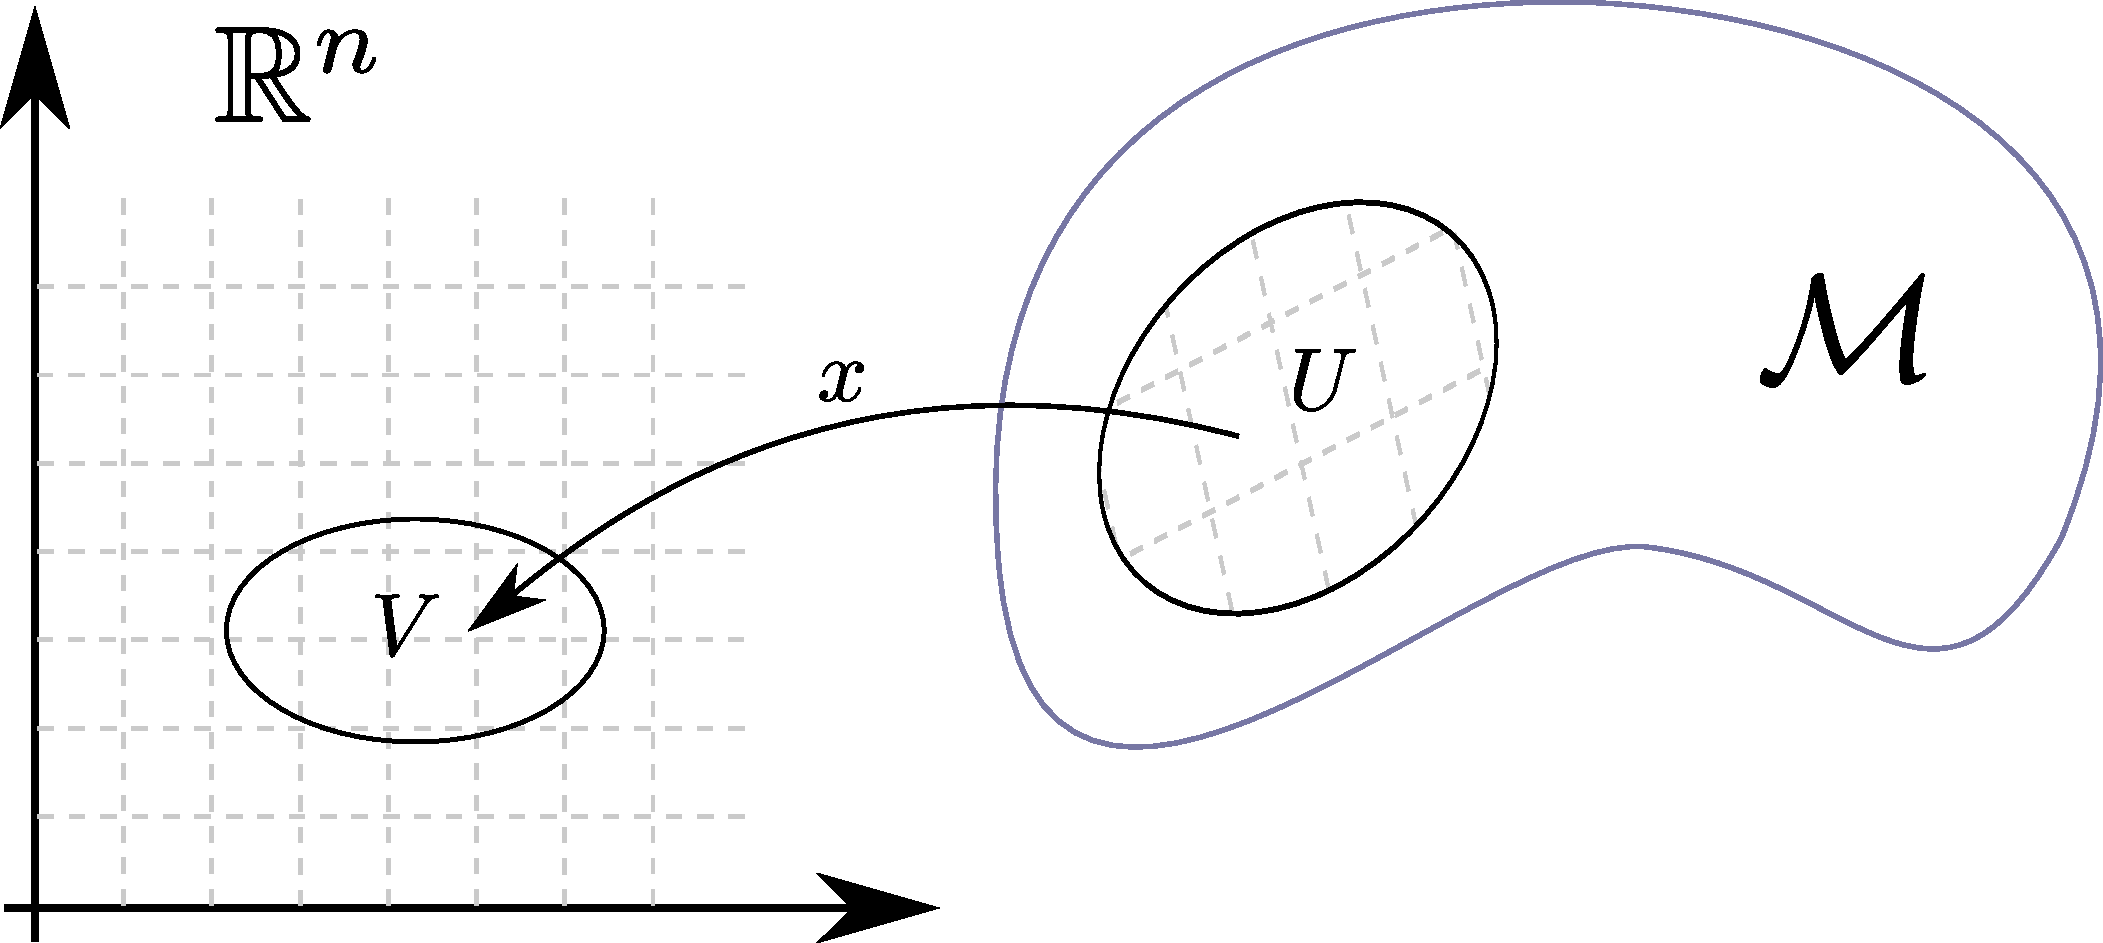
\includegraphics[width=0.7\textwidth]{figurer/coordinate_function.pdf}
    \caption{
        The coordinate function $x$ maps a neighborhood $U$ in the manifold $\Em$ to a neighborhood $V$ in $\R^n$.
        }
    \label{fig: coordinate function}
\end{figure}



This section is taken from my matster's thesis, and is based on~
% autocite{carrollSpacetimeGeometryIntroduction2019,leeIntroductionSmoothManifolds2003d}.


Differential geometry generalizes $n$-dimensional calculus to more general spaces than the usual $\R^n$, such as curved spacetime or the more abstract space of symmetries of a quantum field theory.
The most important objects in differential geometry are \emph{smooth manifolds}.
An $n$-dimensional manifold, $\Em$, is a set of points, locally homeomorphic to $\R^n$.
That is, for all points $p \in \Em$, there exists a neighborhood $U$ around $p$, together with a corresponding set of continuous, bijective functions that map $U$ to a neighborhood $V$ in $\R^n$,
%
\begin{align}
    x: U \subseteq \Em & \longmapsto V \subseteq \R^n, \\
    p & \longmapsto x^\mu(p), \quad \mu \in \{0, \dots, n-1\}.
\end{align}
%
This is illustrated in \autoref{fig: coordinate function}.
We call $x(p) = (x^0(p), \dots, x^{n- 1}(p))$ a coordinate function of $\Em$.
The inverse of $x$, $x^{-1}$, obeys $x^{-1}(x(p)) = p$, for all $p \in U$.
A smooth manifold is one in which the coordinate functions are infinitely differentiable.
To define differentiability on manifolds, consider two coordinate functions, $x$, and $x'$.
The corresponding domains $U$ and $U'$ may or may not overlap.
We then define the transition function, a function between subsets of $\R^n$ by mapping via $\Em$, as
%
\begin{align}
    f_{x'\rightarrow x} = x \circ {x'}^{-1} : \R^n \mapsto \R^n.
\end{align}
%
This map is illustrated in \autoref{fig: transition map}.\footnote{
    To be rigorous, one has to restrict the domains and image of the coordinate function when combining them. This is illustrated in \autoref{fig: transition map}.
    }
A set of coordinate functions $\mathcal A = \{x_i\}$ whose domain cover $\Em$ is called an \emph{atlas} of $\Em$.
If the transition function between all pairings of coordinate functions in the atlas is smooth---that is, infinitely differentiable---we call the atlas smooth.
We then define a smooth manifold as the topological manifold $\Em$ together with a \emph{maximal} smooth atlas $\mathcal A$.
A smooth atlas is maximal if no coordinate function can be added while the atlas remains smooth.\footnote{
    The maximal condition ensures that two equivalent atlases correspond to the same differentiable manifold. A single manifold can be combined with different maximal atlases of smooth coordinates or differentiable structures. A set of examples are \emph{exotic spheres}, smooth manifolds \emph{homeomorphic} to $\text S^n$, but not \emph{diffeomorphic}. 
    }
%
\begin{figure}[!htb]
    \centering
    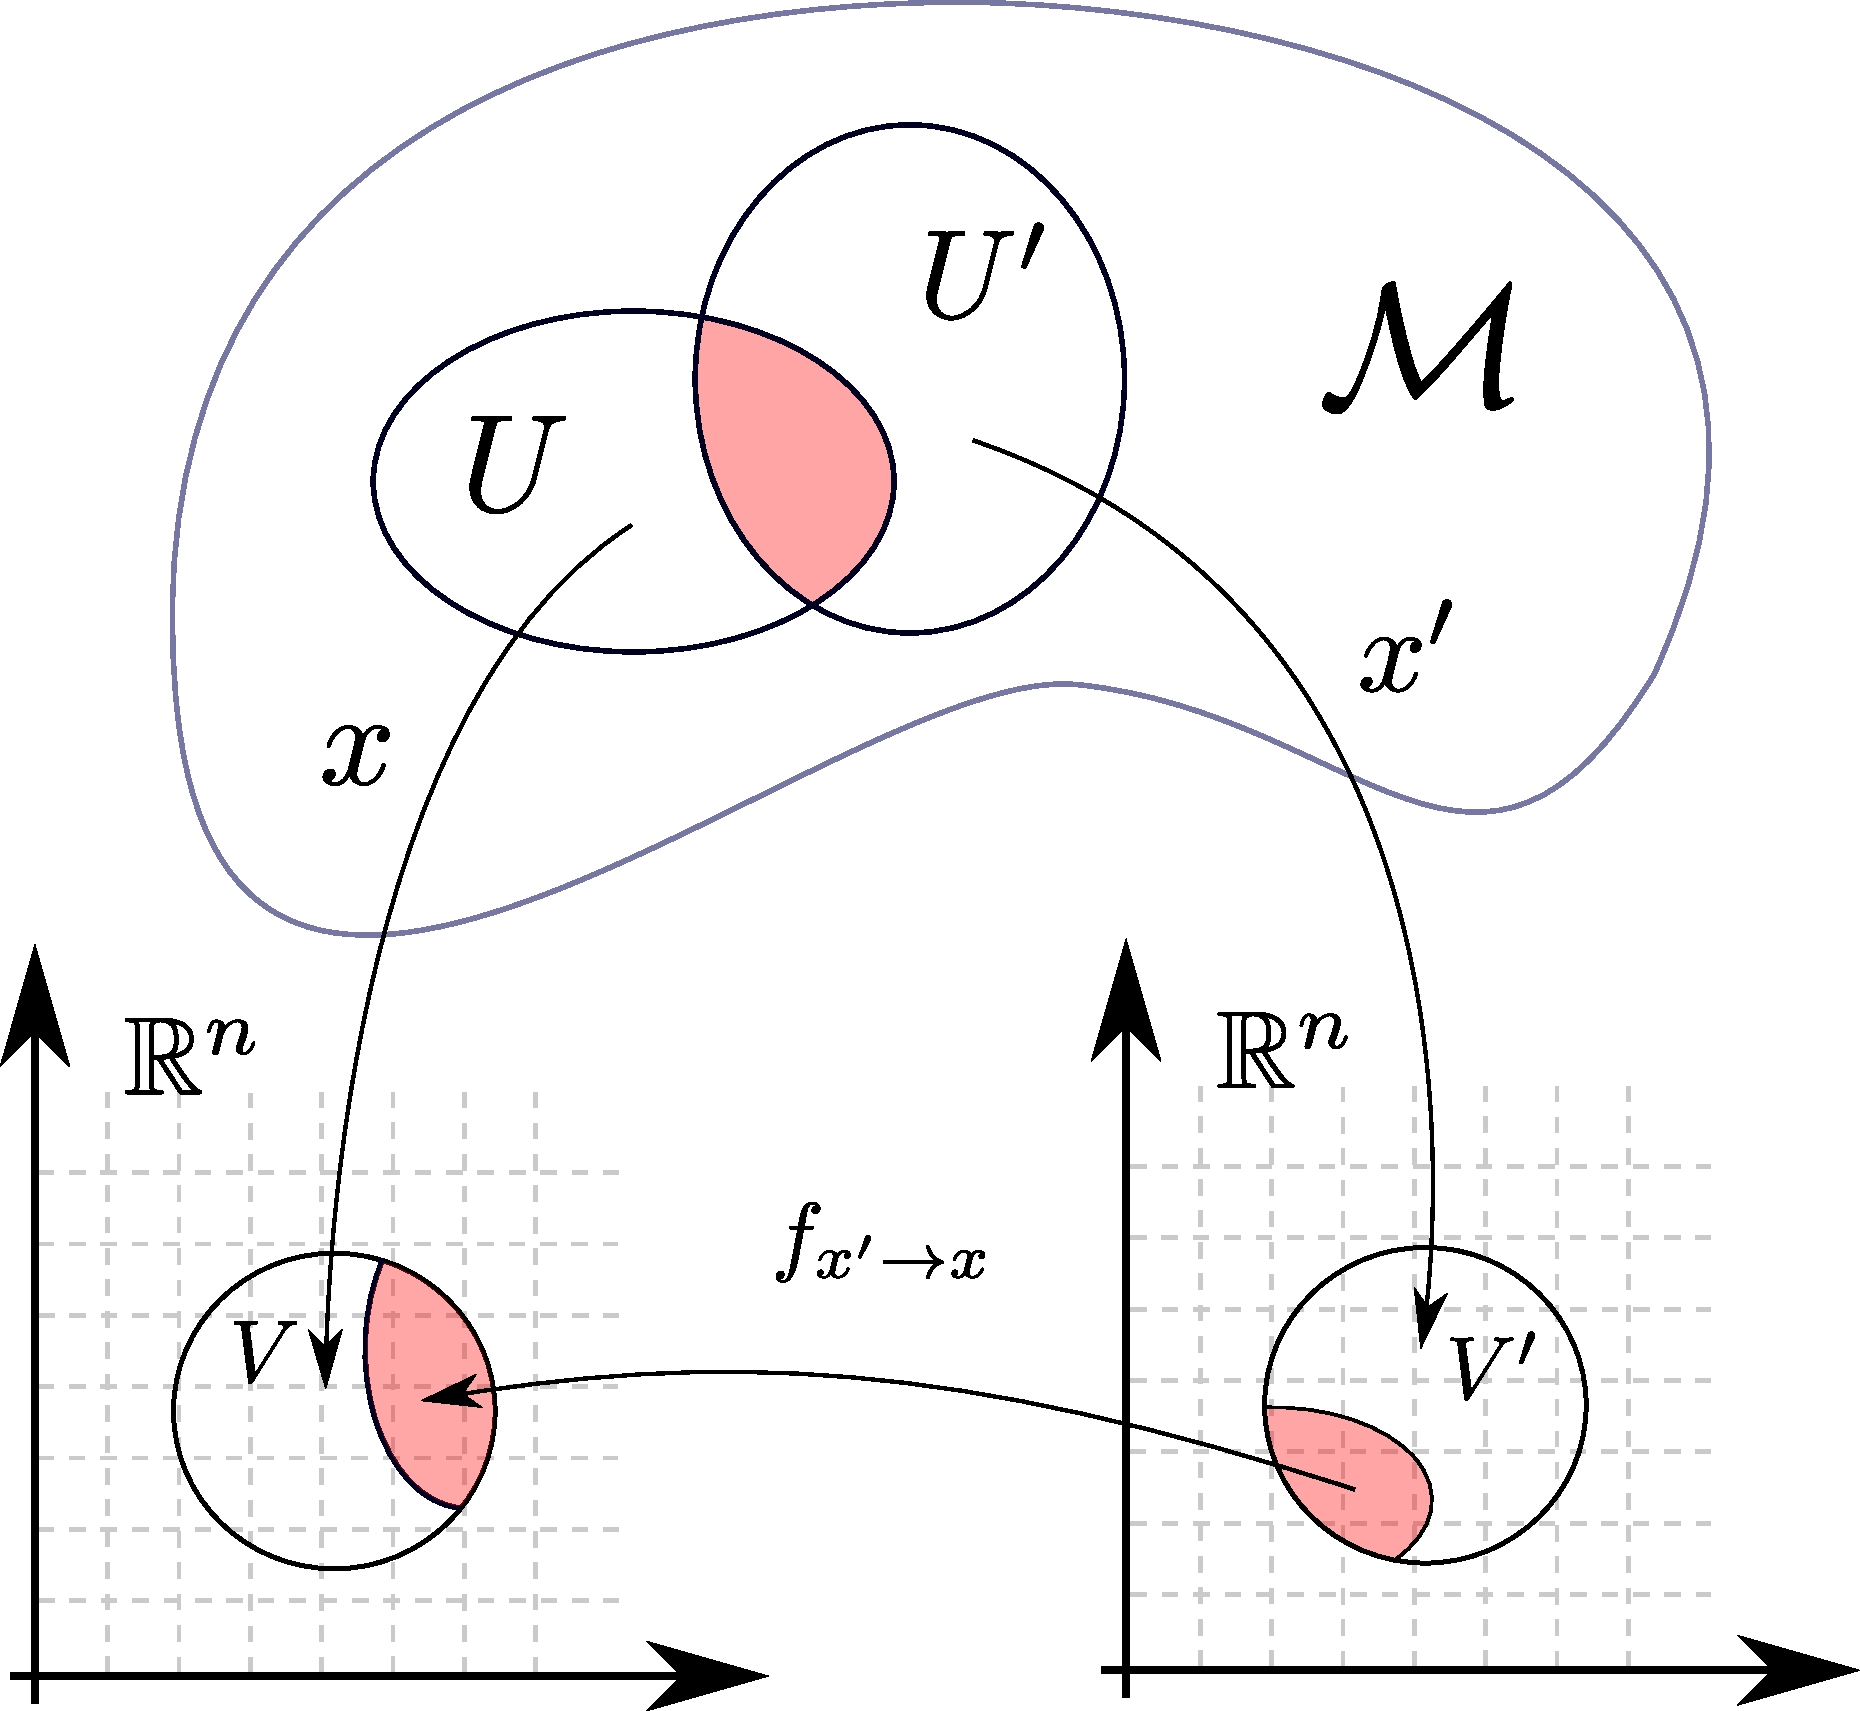
\includegraphics[width=0.6\textwidth]{figurer/transition_map.pdf}
    \caption{
        The transition map $f_{x'\rightarrow x}$ between two coordinate functions, $x'$ and $x$, maps between the images of these function, via the manifold $\Em$. 
        The function's domain and image are restricted to a (possibly empty) subset of the images of $x'$ and $x$. This is illustrated by the shaded regions in $V'$ and $V$. 
        }
    \label{fig: transition map}
\end{figure}

Consider two $m$- and $n$-dimensional smooth manifolds $\Em$ and $\mathcal N$.
Let $x$ denote the coordinates on $\Em$, while $y$ denotes the coordinates on $\mathcal N$.
We can define smooth functions between these manifolds similarly to how we define smooth coordinates.
Consider the function
%
\begin{equation}
    F: \Em \longmapsto \mathcal N.
\end{equation}
%
It is said to be smooth if, for all points $p \in\Em$, there is a set of local coordinates $x$ around $p$ and $y$ around $F(p)$ such that the map $\tilde F = y \circ F \circ x^{-1}$ is smooth.
This map may be illustrated by a diagram,
%
\begin{equation}
    % https://tikzcd.yichuanshen.de/#N4Igdg9gJgpgziAXAbVABwnAlgFyxMJZABgBoBGAXVJADcBDAGwFcYkQAdDgW3pwAsARoIAEAJQB63EAF9S6TLnyEUZYtTpNW7LrwEBjJiICys+SAzY8BIuVLqaDFm0SceffocYiAcmYVWyrYUGk7arroewuIShDIaMFAA5vBEoABmAE4Q0oh2IDgQSGQgjPSCMIwACorWKqUw6TggjlouIAAe-iBZOUj5hUgATK3O7OndvbkjBUWIAMyj4SAAnpPZuSWDC0vtSbKUMkA
\begin{tikzcd}
    \mathcal M \arrow[d, "x"] \arrow[r, "F"] & \mathcal N \arrow[d, "y"] \\
    \mathbb R^m \arrow[r, "\tilde F"]               & \mathbb R^n              
    \end{tikzcd}
    %
\end{equation}
%
%
We will not be careful with the distinction between $F$, the function between the abstract manifolds, and $\tilde F$, the function of their coordinates, but rather denote both by $F(x)$.
We may take the partial derivative of such a function with respect to the coordinates $x$, $\pdv{F}/{x^\mu}$.
However, this is dependent on our choice of coordinates, as a set of local coordinates can always be scaled arbitrarily.
Any physical theory must be independent of our choice of coordinates, so our next task is to define the properties of a smooth manifold in a coordinate-independent way.


\subsection{Vectors and tensors}

A curve $\gamma$ through $\Em$ is a function from $\R$ to $\Em$,
%
\begin{align}
    \gamma : \R &\longmapsto \Em, \\
    \lambda & \longmapsto \gamma(\lambda).
\end{align}
%
Such curves are often denoted only by their coordinates and the parameter $\lambda$, $x^\mu(\lambda) = (x^\mu \circ \gamma)(\lambda)$.
With this curve, we can take the directional derivative of a real-valued function on the manifold, $f: \Em \mapsto \R$.
Assume $\gamma(\lambda = 0) = p$.
As we are always taking the derivative of functions between $\R^n$, for different $n$, we can use the chain rule.
The directional derivative of $f$ at $p$, given by this curve $\gamma$, is then
%
\begin{equation}
    \odv{}{\lambda} f(x(\lambda)) \bigg |_p = \odv{x^\mu}{\lambda} \bigg |_{\lambda = 0}  \pdv{}{x^\mu} f(x) \bigg |_p.
\end{equation}
%
The set of all such directional derivatives, $\odv{}/{\lambda}$ at $p$, form a vector space, $T_p \Em$, called the \emph{tangent space}.
The tangent space is illustrated in \autoref{fig: tangent space}.


\begin{figure}[!htb]
    \centering
    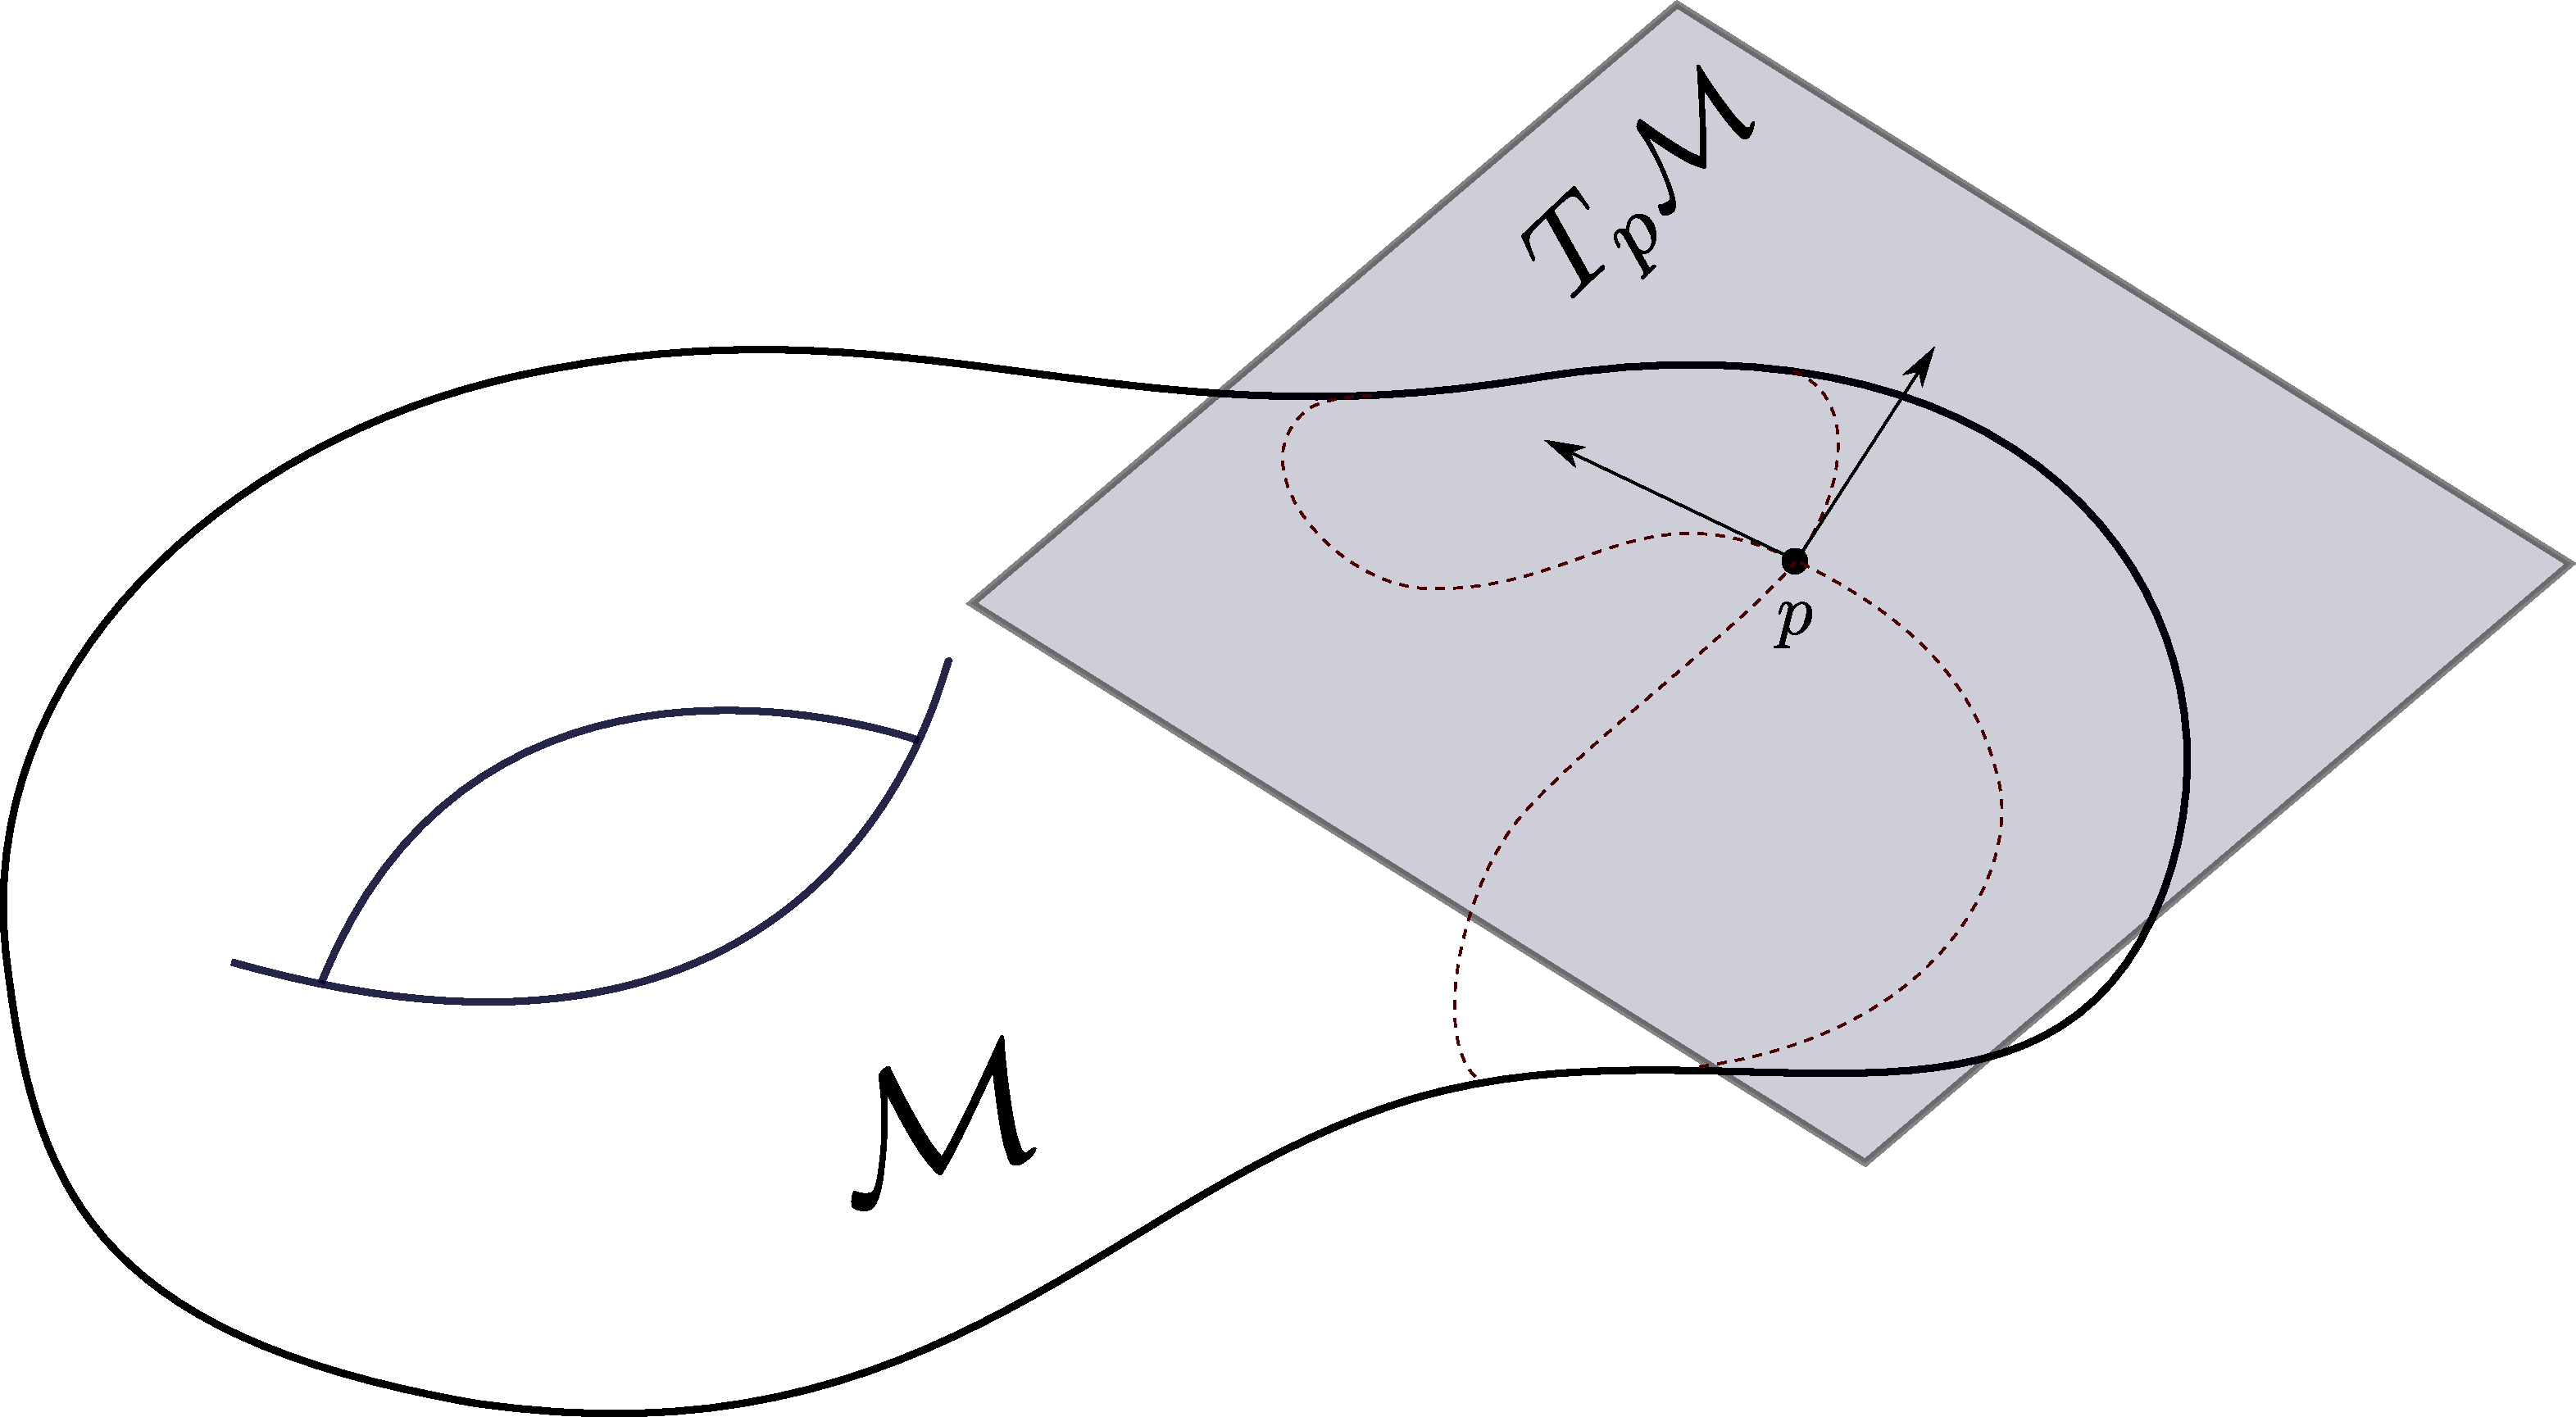
\includegraphics[width=0.7\textwidth]{figurer/tangent space.pdf} 
    \caption{
        The tangent space $T_p \Em$, the shaded rectangle, is the sett of all directional derivatives at $p\in \Em$. A directional derivative is defined in terms of a curve that passes through $p$.
        } 
    \label{fig: tangent space}
\end{figure} 


The coordinates $x^\mu$ induce a basis of this vector space, namely partial derivatives with respect to the coordinate functions at $p$,
%
\begin{equation}
    e_\mu = \pdv{}{x^\mu} \bigg|_p = \partial_\mu|_p, \quad \mu \in \{0, ... n-1\}.
\end{equation}
%
Any element $v \in T_p \Em$ can therefore be written
%
\begin{equation}
    v = v^\mu \partial_\mu |_p = \odv{x^\mu}{\lambda}\Big |_{\lambda = 0} \pdv{}{x^\mu}\Big |_p.
\end{equation}
%
Here, $\lambda$ is the parameter of the curve corresponding to the directional derivative $v$.\footnote{%
There is not only one curve corresponding to any directional derivative but rather an equivalence class. We will gloss over this technicality, as it does not affect our work.
}
The evaluation at $\lambda = 0$ and $p$ will often be implicit for ease of notation.
This directional derivative acts on functions $f : \Em \mapsto \R$ as
%
\begin{equation}
    v(f) = v^\mu \partial_\mu f.
\end{equation}
%




A map $F$ between two manifolds $\Em$ and $\mathcal N$ also induces a map between the tangent spaces of these manifolds.
This is the \emph{differential} of $F$ at $p$, 
%
\begin{align}
    \dd F_p: T_p \Em & \longmapsto T_p \mathcal N, \\
    v & \longmapsto \dd F_p (v). 
\end{align}
%
$\dd F_p(v)$ is an element of $T_p \mathcal N$, i.e., it is a directional derivative on $\mathcal N$.
It is defined by how it acts on functions $g: \mathcal N \mapsto \R$,
%
\begin{equation}
    \dd F_p(v) (g) = v(g \circ F),
\end{equation}
%
It thus acts on functions on $\mathcal N$ by ``extending'' the derivative $v$.
This is a linear map between vector spaces and may be written in component form by considering the differentials of the coordinate functions.
Denote the coordinates of $\mathcal N$ by $y^\mu$, and $y^\mu \circ F = F^\mu$.
Then,
%
\begin{equation}
    \dd F_p (\partial_\mu) (g) = \partial_\mu (g \circ F) |_p 
    = \pdv{F^\nu}{x^\mu}\Big |_p \pdv{g}{y^\nu} \Big  |_{F(p)},
\end{equation}
%
or more suggestively
%
\begin{equation}
    \dd F \left( \pdv{}{x^\mu} \right) = \pdv{F^\nu}{x^\mu} \pdv{}{y_\nu}.
\end{equation}
%
This is a linear map of vectors between two vectors by the matrix $A_\mu{}^\nu = \partial_\mu F^\nu$.
The differential is thus a generalization of the Jacobian.
In the case of a real valued function, $f: \Em \mapsto \R$, and $g : \R \mapsto \R$, we get
%
\begin{equation}
    \dd f (v) (g) 
    = v(g \circ f) 
    = (v^\mu \partial_\mu f) \, \odv{g}{y}.
\end{equation}
%
$\dd f$ is thus a map from $T_p \Em$ to $T_{f(p)}\R$, which is isomorphic to $\R$.
Let $g$ be the identity function, so that $\odv{g}/{y} = 1$.
Then, the differential of a scalar function, also called a 1-form, is a map from vectors $v$ to real numbers,
%
\begin{equation}
    \label{covectors i.e. one forms}
    \dd f(v) := v^\mu \partial_\mu f.
\end{equation}
%
The set of all linear maps from a vector space $V$ to the real numbers is called the \emph{dual space} of $V$, denoted $V^*$.
This is a new vector space with the same dimensionality as $V$.
We denote the dual of $T_p \Em$ as $T_p^* \Em$.
We can regard each coordinate function as a real-valued function with a corresponding differential.
This differential obeys
%
\begin{equation}
    \dd x^\mu (\partial_\nu) = \pdv{x^\mu}{x_\nu} = \delta^\mu_\nu.
\end{equation}
%
The differentials of the coordinate functions thus form a basis for $T^*_p \Em$, called the dual basis.
Any differential $\dd f$ can thus be written as $\dd f = \omega_\mu \dd x^\nu$ for some components $\omega_\mu$.
We finde the components by applying the differential to the coordinate basis, $\dd f(\partial_\mu) = \partial_\mu f = \omega_\mu$.
In other words, we recover the classical expression 
%
\begin{equation}
    \dd f = \pdv{f}{x^\mu} \dd x^\mu,
\end{equation}
however we now interpret it as a covector-field instead of an ``infinitesimal displacement''.

Linear maps from vectors to real numbers is generalized by \emph{tensors}.
Given a vector space $V$, a general $(n, m)$ tensor $T$ is a multilinear map, which associates $n$ elements from $V$ and $m$ from its dual $V^*$ to the real numbers, i.e.,
%
\begin{align}
    T: V \times V \times \dots\times V^* \times \dots &\longmapsto \R, \\
    (v, u\dots; \omega, \dots) & \longmapsto T(v, u, \dots; \omega, \dots).
\end{align}
%
Multilinear means that $T$ is linear in each argument.
The set of all such maps is the tensor product space $V\otimes V \otimes \dots \otimes V^* \otimes \dots$, a $\dim(V)^{n+m}$-dimensional vector space.
If $\{e_\mu\}$ and $\{e^\mu\}$ are the basis for $V$ and $V^*$, then we can write the basis of this of the tensor product space as $ \{e_{\mu} \otimes \dots \otimes e^{\nu} \otimes \dots \}$.
The tensor can thus be written
%
\begin{equation}
    T =
     T^{\mu \nu\dots}{}_{\rho\dots} \, e_{\mu}\otimes e_\nu \otimes \dots e^\rho\otimes\dots, \quad
    T^{\mu \nu\dots}{}_{\rho\dots} = T(e^\mu, e^\nu, \dots; e_\rho, \dots).
\end{equation}
% 
We often want to decompose a tensor down into its symmetric and antisymmetric parts.
To do this, we introduce the symmetrization of a tensor $T$, 
%
\begin{equation}
    T_{(\mu_1\dots\mu_n)} 
    = \frac{1}{n!} \sum_{\sigma \in S_n} 
    T_{\mu_{\sigma(1)} \dots \mu_{\sigma(n)}},
\end{equation}
%
where $S_n$ is the set of all permutations of $n$ objects.
The antisymmetrization of a tensor is defined as
%
\begin{equation}
    T_{[\mu_1\dots\mu_n]} 
    = \frac{1}{n!} \sum_{\sigma \in S_n} \text{sgn}(\sigma)  
    T_{\mu_{\sigma(1)} \dots\mu_{\sigma(n)}}.
\end{equation}
%
The function $\text{\sigma} = \pm 1$, depending on if $\sigma$ is a even or odd permutation.
We may now write
%
\begin{equation}
    T_{\mu \nu} = T_{(\mu \nu)} + T_{[\mu \nu]}.
\end{equation}




\subsection{Geometry and the metric}
\label{subsection: goemetry and the metric}

The metric is a symmetric, non-degenerate $(0, 2)$ tensor
%
\begin{equation}
    \dd s^2 = g_{\mu \nu} \, \dd x^\mu \otimes \dd x^\nu.
\end{equation}
%
It defines the geometry of the manifold $\Em$ and is the main object of study in general relativity.
As it is invertible, we can define $g^{\mu \nu} = (g^{-1})_{\mu \nu}$, which is the components of a $(2, 0)$ tensor.
We use this to raise and lower indices, as is done with the Minkowski metric $\eta_{\mu \nu}$ in special relativity.

Up until now, we have only considered the tangent space $T_p \Em$ at a point $p$ and the corresponding tensor-product spaces.
We are, however, more interested in \emph{fields} of vectors, covectors, or tensors.
For each point $p \in \Em$, a tensor field $T$ ``picks out'' a tensor $T(p)$ from each tensor product space corresponding to the tangent space at $p$, $T_p \Em$.
A vector field can be written as
%
\begin{equation}
    v(p) = v^\mu(p) \partial_\mu |_p. 
\end{equation}
%
We will mostly be working with the components $v^\mu$, which are functions of $\Em$.
For ease of notation, we write the vector as a function of the coordinates $x$.
The vector field $v(x)$ is unchanged by a coordinate-transformation $x^\mu \rightarrow {x'}^\mu$; the coordinates are only a tool for our convenience.
However, with a new set of coordinates, we get a new set of basis vectors, $\partial'_\mu$:
%
\begin{equation}
    v = v^\mu \partial_\mu = v^\mu \pdv{x'^\nu}{x^\mu} \partial'_\nu
    = v'^\mu \partial_\mu',
\end{equation}
%
This gives us the transformation rules for the components of vectors,
%
\begin{equation}
    v'^\mu = \pdv{x'^\mu}{x^\nu} v^\nu.
\end{equation}
%
Tangent vectors are also called \emph{contravariant} vectors, as their components transform contra to the basis vectors.
For covectors, it is
%
\begin{equation}
    \omega'_\mu = \omega_\nu \pdv{x^\nu}{x'^\mu},
\end{equation}
%
which is why covectors also are called \emph{covariant} vectors.

The gradient of a scalar function $f$, $\dd f = \partial_\mu f \dd x^\mu$, is a coordinate-independent derivative, as $\partial_\mu f$ follows the transformation law for covectors.
To generalize this, we define the covariant derivative, $\nabla$, as a map from $(n, m)$ tensor fields to $(n, m+1)$ tensor fields, as $f\rightarrow\dd f$ maps a $(0,0)$ tensor, a scaalar, to a $(0,1)$- tensor
The components of a covariant derivative, $\nabla_\rho T^{\mu_1\dots}{}_{\nu_1, \dots}$, must follow the tensor transformation law. 
However, this is not strong enough to uniquely define $\nabla$.
In addition to $\nabla f = \partial f$, we further assume the derivative is linear, $\nabla (T + S) = \nabla T + \nabla S$, and follow the product rule: $\nabla (T \otimes S) = (\nabla T)\otimes S + T \otimes (\nabla S)$.
Lastly, we assume the derivative of the Kronecker delta gives zero, $\nabla_\mu \delta^\rho_\nu = 0$.
With this, we can, in general, write the covariant derivative for vectors and covectors as~\autocite{carrollSpacetimeGeometryIntroduction2019}
%
\begin{align}
    \label{covariant derivative diff geom}
    \nabla_\mu v^\nu &= \partial_\mu v^\nu + \Gamma^\mu_{\nu \rho} v^\rho, \\
    \label{covariant derivative diff geom covector}
    \nabla_\mu \omega_\nu &= \partial_\mu \omega_\nu - \Gamma^\rho_{\mu \nu} \omega_\rho.
\end{align}
%
$\Gamma^{\mu}_{\nu \rho}$ are called \emph{Christoffel symbols}.
The generalization for higher-order tensors is straightforward, 
%
\begin{equation}
    \nabla_\mu T^{\nu\dots}{}_{\rho\dots}
    =
    \partial_\mu T^{\nu\dots}{}_{\rho\dots}
    + \Gamma^\mu_{\nu \lambda} T^{\lambda\dots}{}_{\rho\dots} +\dots
    - \Gamma^\lambda_{\mu \rho} T^{\mu\dots}{}_{\lambda\dots} -\dots.
\end{equation} 
%
This is still not enough to uniquely determine the covariant derivative.
We will furthermore assume $\Gamma^{\lambda}_{\mu \nu} = \Gamma^{\lambda}_{\nu \mu}$ and $\nabla_\mu g_{\nu \rho} = 0$.
With these assumptions, we find an explicit formula of the Christoffel symbols in terms of the metric,
%
\begin{equation}
    \label{christoffel symbols from metric}
    \Gamma^\rho_{\mu \nu} = \frac{1}{2} g^{\rho \sigma} (\partial_\mu g_{\nu \sigma} - \partial_\sigma g_{\mu \nu} + \partial_{\nu}g_{\sigma \mu}).
\end{equation}
%
Using the notion of a covariant derivative, we may also generalize \emph{parallel transport} to curved spaces.
The notion of parallel transport of a vector in flat $\R^n$ is intuitive---given a line $x^\mu(\lambda)$, a vector $v^\mu$ at $x^\mu(\lambda_0)$ is parallel transported to $v'^\mu$ at $x^\mu(\lambda_1)$ if you carry it along the line without ``turning it''.
To make this more precise, a vector field $v^\mu$ is parallel transported along $x^\mu(\lambda)$ if $\odv{}{\lambda} v^\mu = \odv{x^\nu}{\lambda} \partial_\nu v^\mu$ = 0.
We generalize this to curved spaces by replacing the partial derivative with a covariant derivative, and so the criterion for parallel transport is
%
\begin{equation}
    \label{parallel transport criterion}
    \odv{x^\mu}{\lambda} \nabla_\mu v^\nu = 0.
\end{equation}
%
With this, we can imagine creating a special class of paths, called \emph{geodesics}, namely those which parallel transport their tangent vectors $\odv{x^\mu}{\lambda}$.
We imagine following an arrow we are holding without turning it as we walk.
Using the definition of parallel transport \autoref{parallel transport criterion}, together with the covariant derivative \autoref{covariant derivative diff geom}, we get the geodesic equation,
%
\begin{equation}
    \label{goedesic equation}
    \odv[2]{x^\mu}{\lambda} 
    + \Gamma^\mu_{\rho \sigma} \odv{x^\rho}{\lambda} \odv{x^\sigma}{\lambda}
    = 0.
\end{equation}
In a flat space, where the Christoffel symbols vanish, this reduces to the familiar criterion for straight lines, $\odv[2]{x^\mu}{\lambda} = 0$.

The curvature of a manifold $\Em$, with the metric $g_{\mu \nu}$, is encoded in the Riemann tensor.
It is defined by
%
\begin{equation}
    \label{Riemann tensor}
    [\nabla_\mu, \nabla_\nu] v^\rho = R^{\rho}{}_{\sigma \mu \nu} v^\sigma,
\end{equation}
%
which, in our case, gives the explicit formula
%
\begin{equation}
    \label{riemann tensor in terms of christoffel symbols}
    R^\rho{}_{\sigma \mu \nu} 
    = \partial_{\mu} \Gamma^{\rho}_{\nu \sigma}
    - \partial_{\nu} \Gamma^{\rho}_{\mu \sigma}
    + \Gamma^{\rho}_{\mu \lambda} \Gamma^{\lambda}_{\nu \sigma}  
    - \Gamma^{\rho}_{\nu \lambda} \Gamma^{\lambda}_{\mu \sigma}.
\end{equation}
%
This form of the Riemann tensor allows us to derive several useful identities, such as
%
\begin{equation}
    R_{\rho \sigma \mu \nu} 
    = 
    R_{[\rho \sigma] \mu \nu}
    =
    R_{\rho \sigma [\mu \nu]}
    =
    R_{\mu \nu \rho \sigma }.
\end{equation}
%
In addition, the properties of the commutator imply the Jacobi identity,
%
\begin{equation}
    \label{Jacobi identity differential geometry}
    [\nabla_\mu, [\nabla_\nu, \nabla_\sigma]]
    + [\nabla_\sigma, [\nabla_\mu, \nabla_\nu]]
    + [\nabla_\nu, [\nabla_\sigma, \nabla_\mu]] = 0.
\end{equation}
%
If we apply this on $\delta^{\mu}_{\nu}$, we get the differential Bianchi identity, compactly written
%
\begin{equation}
    \label{Binachi identiy}
    \nabla_{[\mu}R_{\nu \rho]\sigma \eta} = 0.
\end{equation}
%
Although the Christoffel symbols are not tensors, the Riemann tensor is, due to its definition using covariant derivatives.
We can therefore contract some of its indices to get other tensorial quantities.
We define the Ricci tensor and Ricci scalar as
%
\begin{align}
    \label{Ricci tensor}
    R_{\mu \nu} &= R^{\rho}{}_{\mu \rho \nu}, \\
    \label{Ricci scalar}
    R &= R^{\mu}{}_{\mu} = g^{\mu \nu} R_{\mu \nu}.
\end{align}


To interpret the Riemann tensor, we define the parallel propagator $P$.
We want this object to take a vector at one point and parallel transport it to another point.
A vector that is transported along a curve parametrized by $\lambda$ should then obey
%
\begin{equation}
    v^\mu(\lambda) = P^\mu{}_\nu(\lambda) v^\nu.
\end{equation}
%
Inserting this into the equation for parallel transport, \autoref{parallel transport criterion}, this operator must obey
%
\begin{equation}
    \odv{}{\lambda} P^\mu{}_\nu = - \Gamma^\mu_{\rho \sigma}  \odv{x^\rho}{\lambda}P^\sigma{}_\nu.
\end{equation}
%
This has the same form as the definition of the unitary time-evolution operator in quantum mechanics, and we could therefore write down a solution involving an exponential and a path ordering operator, $\mathcal P$, analogous to the time ordering operator from quantum mechanics.
We may rewrite the equation on an integral form,
%
\begin{equation}
    P^\mu{}_\nu(\lambda) = \delta^\mu_\nu 
    - \int^\lambda_0 \dd \lambda' \Gamma^\mu_{\rho \sigma} V^\rho P^\sigma{}_\nu,
\end{equation}
%
where we denote $\odv{x^\mu}{\lambda} = V^\mu$.
This allows us to solve the equation iteratively.
If $\lambda \leq \epsilon \ll 1$, we expect this to converge as long as the $g$ is well-behaved.
Starting with the zeroth-order solution $P^{\mu}{}_\nu = \delta^\mu_\nu$ and iterating twice gives us
%
\begin{equation}
    \label{iterative paralell propagator}
    P^\mu{}_\nu(\lambda) 
    = 
    \delta^\mu_\nu 
    - \int_0^\lambda \dd \lambda' \, 
    \Gamma^\mu_{\rho \nu} V^\rho
    + \int_0^{\lambda} \dd \lambda ' \int_0^{\lambda'} \dd \lambda ''\,
    \Gamma^\mu_{\rho \sigma} \Gamma^\sigma_{\eta \nu} V^\rho V^\eta
    + \Oh(\epsilon^3).
\end{equation}
%
With this, we will investigate how much a vector $v^\mu$ is changed by being parallel transported around in a small loop, as illustrated in \autoref{fig: parallel transport in loop}.

\begin{figure}[!htb]
    \centering
    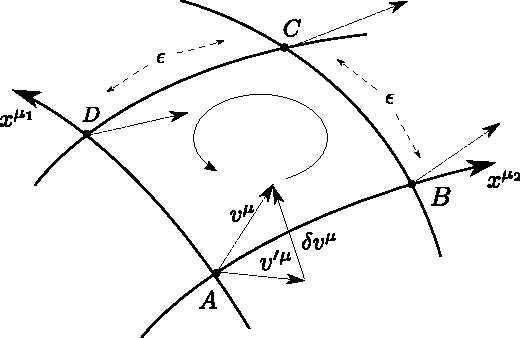
\includegraphics[width=0.6\textwidth]{figurer/parallel_transport.pdf}
    \caption{A vector $v^\mu$ is parallel transported in a small, closed loop, defined by the coordinate functions $x^{\mu_1}$ and $x^{\mu_2}$.
    As a consequence of the curvature, it has changed by $\delta v^\mu$ by the time it arrives back at $A$.}
    \label{fig: parallel transport in loop}
\end{figure}


We transport $v^\mu$ along the coordinate lines.
These are lines where either of the coordinate functions $x^{\mu_1}$ or $x^{\mu_2}$ are equal to $0$ or $\epsilon$.
Here, the indices $\mu_1$ and $\mu_2$ are not free but identify the two coordinate functions which define this loop.
They will therefore break summation rules; such indices may appear only on one side of an equation.
The line from $A$ to $B$, defined by $x^{\mu_1} = 0$, is parametrized by $x^\mu(\lambda) = \lambda \delta^\mu_{\mu_2}$, so $ V^\mu = \delta^\mu_{\mu_2} $.
The Christoffel symbol along this line is
%
\begin{equation}
    \Gamma^{\mu}_{\nu \rho}(\lambda) 
    = \Gamma^{\mu}_{\nu \rho}|_A
    + \lambda \partial_{\mu_2} \Gamma^{\mu}_{\nu \rho}|_A + \Oh(\epsilon^2).
\end{equation}
%
Inserting this into \autoref{iterative paralell propagator}, we get
%
\begin{equation}
    P^\mu{}_\nu(\epsilon)
    = \delta^\mu_\nu 
    - \epsilon \Gamma^{\mu}_{\nu \mu_2}|_A
    + \frac{1}{2} \epsilon^2 
    \left(
        \Gamma^\mu_{\mu_2 \sigma}\Gamma^\sigma_{\mu_2 \nu} |_A 
        -\partial_{\mu_2} \Gamma^{\mu}_{\nu \mu_2}|_A 
    \right)
    + \Oh(\epsilon^3).
\end{equation}
%
Next, from $B$ to $C$, the line is $x^\mu(\lambda) = \epsilon \delta^\mu_{\mu_2} + \lambda \delta^{\mu}_{\mu_1}$, so $V^\mu = \delta^\mu_{\mu_1}$, and the Christoffel symbols are 
$ 
\Gamma^{\mu}_{\nu\rho}
= 
\Gamma^{\mu}_{\nu \rho}|_B
+ \lambda \partial_{\mu_1} \Gamma^{\mu}_{\nu \rho}|_B
$
to fist order in $\lambda$.
Here, we have to expand once more to evaluate the symbols at $A$.
Then, we get
%
\begin{equation}
    \Gamma^{\mu}_{\nu\rho}
    =
    \Gamma^{\mu}_{\nu \rho}|_A + \epsilon \partial_{\mu_2} \Gamma^{\mu}_{\nu \rho}|_A
    + \lambda \partial_{\mu_1} \Gamma^{\mu}_{\nu \rho}|_A + \Oh(\epsilon^2),
\end{equation}
%
The parallel propagator from $B$ to $C$ is then
%
\begin{equation}
    P^{\mu}{}_\nu(\epsilon)
    = 
    \delta^\mu_\nu
    - \epsilon \Gamma^{\mu}_{\nu \mu_1}|_A 
    + \frac{1}{2}\epsilon^2
    \left(
        \Gamma^\mu_{\sigma \mu_1}\Gamma^\sigma_{\nu \mu_1}|_A
        - \partial_{\mu_1} \Gamma^{\mu}_{\nu \mu_1}|_A
        - 2 \partial_{\mu_2} \Gamma^{\mu}_{\nu \mu_1}|_A
    \right)
    + \Oh(\epsilon^3),
\end{equation}
%
Which gives the combined propagator from $A$ to $C$, to and including second order in $\epsilon$, as
%
\begin{align}
    \nonumber
    {P_{AC}}^\mu{}_{\nu}
    & = 
    \left[ 
        \delta^\mu_\sigma 
        -\epsilon \Gamma^{\mu}_{\sigma \mu_1}
        + \frac{1}{2} \epsilon^2 
        \left(
        \Gamma^\mu_{\eta \mu_1}\Gamma^\eta_{\sigma \mu_1}
        - \partial_{\mu_2} \Gamma^{\mu}_{\sigma \mu_2}
        - 2 \partial_{\mu_2} \Gamma^{\mu}_{\sigma \mu_1}
        \right)
    \right]\\\nonumber
    &\quad\times
    \left[
        \delta^\sigma_\nu
        - \epsilon \Gamma^{\sigma}_{\nu \mu_2}
        + \frac{1}{2} \epsilon^2 
        \left(
            \Gamma^\sigma_{\eta \mu_2}\Gamma^\eta_{\nu \mu_2}
            - \partial_{\mu_2} \Gamma^{\sigma}_{\nu \mu_2}
        \right)
    \right] \\ \nonumber
    & =
    \delta^\mu_\nu
    - \epsilon 
    \left(
        \Gamma^{\mu}_{\nu \mu_1}
        +
        \Gamma^{\mu}_{\nu \mu_2}
    \right)\\
    &\quad
    + \epsilon^2
    \frac{1}{2}
    \left(  
        2\Gamma^{\mu}_{\sigma \mu_1} \Gamma^{\sigma}_{\nu \mu_2}
        + \Gamma^\mu_{\sigma \mu_1}\Gamma^\sigma_{\nu \mu_1}
        + \Gamma^\mu_{\sigma \mu_2}\Gamma^\sigma_{\nu \mu_2}
        - 2 \partial_{\mu_2} \Gamma^{\mu}_{\nu \mu_1}
        - \partial_{\mu_1} \Gamma^{\mu}_{\nu \mu_1}
        - \partial_{\mu_2} \Gamma^{\mu}_{\nu \mu_2}
    \right).
\end{align}
%
The parallel propagator for $CDA$ is the propagator for $ADC$ with its signs flipped. 
The $ADC$ propagator is the same as $ABC$, only with the $\mu_1$ and $\mu_2$ indices switched.
It is thus
%
\begin{align}
    \nonumber
    {P_{CA}}^\mu{}_\nu
    & =
    \delta^\mu_\nu
    + \epsilon 
    \left(
        \Gamma^{\mu}_{\nu \mu_2}
        +
        \Gamma^{\mu}_{\nu \mu_1}
    \right)\\
    &\quad
    + \epsilon^2
    \frac{1}{2}
    \left(  
        2\Gamma^{\mu}_{\sigma \mu_2} \Gamma^{\sigma}_{\nu \mu_1}
        + \Gamma^\mu_{\sigma \mu_2}\Gamma^\sigma_{\nu \mu_2}
        + \Gamma^\mu_{\sigma \mu_1}\Gamma^\sigma_{\nu \mu_1}
        + 2 \partial_{\mu_1} \Gamma^{\mu}_{\nu \mu_2}
        + \partial_{\mu_2} \Gamma^{\mu}_{\nu \mu_2}
        + \partial_{\mu_1} \Gamma^{\mu}_{\nu \mu_1}
    \right).
\end{align}
%
The full propagator, from $A$ to $A$, is $P^\mu{}_\nu = {P_{CA}}^\mu{}_\rho {P_{AC}}^\rho{}_\nu$.
The terms linear in $\epsilon$ vanish, and the same with the terms with two equal $\mu_i$-indices.
The change in the vector as it is rotated around the loop is therefore, to second order in $\epsilon$,
%
\begin{align}
    \delta v^\mu 
    = P^\mu{}_\nu v^\nu - v^\mu 
    = \epsilon^2  
    \left(
        \Gamma^\mu_{\sigma \mu_1} \Gamma^\sigma_{\nu \mu_2}
        -\Gamma^\mu_{\sigma \mu_2} \Gamma^\sigma_{\nu \mu_1}
        + \partial_{\mu_1} \Gamma^{\mu}_{\nu \mu_2}
        - \partial_{\mu_2} \Gamma^{\mu}_{\nu \mu_1} 
    \right) v^\nu.
\end{align}
Comparing with \autoref{riemann tensor in terms of christoffel symbols}, we see that this is the Riemann curvature tensor.
In other words, the Riemann tensor encodes how a vector is transformed when parallel transported in a small, closed loop.



\subsection{Integration on manifolds}
\label{subsection: integration on manifolds}

The integral of a scalar function on a manifold is not a coordinate-independent notion.
To obtain this, we must introduce $n$-forms.
A $n$-form $\omega$ is an antisymmetric $(0, n)$ tensor.
This means that it has coordinates which obey $\omega_{\mu_1 \dots \mu_n} = \omega_{[\mu_1 \dots \mu_n]}$.
The $n$-forms are ubiquitous objects in mathematics and physics, one example is the electromagnetic field-strength tensor $F_{\mu \nu}$, and they allow for the definitions of coordinate independent integration and derivation.
We will define two important maps between $n$-forms.
The wedge product, $\wedge$, is a product that maps two $n$- and $m$-forms to an $n+m$-form, and is defined as
%
\begin{equation}
    (A\wedge B)_{\mu_1\dots\mu_{n+m}} = \frac{(n + m)!}{n! m!} A_{[\mu_1\dots\mu_n}B_{\mu_{n+1}\dots\mu_{n+m}]}.
\end{equation}
%
Furthermore, we define the exterior derivative, a map from $n$-forms to $n+1$-forms, defined by
%
\begin{equation}
    (\dd T)_{\mu_1 \dots \mu_{n+1}} = (n+1) \partial_{[\mu_1} T_{\mu_2\dots\mu_{n+1}]}.
\end{equation}
%
We are interested in a coordinated independent quantity that we can integrate over.
To that end, we define
%
\begin{equation}
    \dd^n x := \dd x^0 \wedge \dots \wedge \dd x^{n-1}
    = \varepsilon_{\mu_1 \dots \mu_n}  
    \dd x^{\mu_1} \otimes \dots \otimes \dd x^{\mu_n},
\end{equation}
%
where $\varepsilon_{\mu_1 \dots \mu_n}$ is the Levi-Civita symbol.
Given a new set of coordinates, $x'^\mu$, we may similarly define a new $n$-form, $\dd^n x'$.
These two $n$-forms are related by
%
\begin{equation}
    \dd^n x = \det\left( \pdv{x}{x'} \right) \, \dd^n x',
\end{equation}
%
where we have used the relation $\varepsilon_{\mu_1 \dots \mu_n}  \det(A) = \varepsilon_{\nu_1 \dots \nu_n} A^{\nu_1}{}_{\mu_1} \dots A^{\nu_n}{}_{\mu_n}$.  
We define $|g| = |\det(g_{\mu \nu })|$, where $|\cdot|$ denote the absolute value.
By the transformation properties of tensors, this transforms as
%
\begin{equation}
    \sqrt{|g'|} = \left| \det\left(\pdv{x'}{x} \right) \right| \sqrt{|g'|},
\end{equation}
%
This means we can use $|g|$ to compensate for the transformation of $\dd^n x$, and get a volume form with a coordinate independent definition,
%
\begin{equation}
    \dd V = \sqrt{|g|} \, \dd^n x = \sqrt{|g'|} \, \dd^n x'.
\end{equation}
%
With this, we can integrate scalars in a well-defined way by mapping them to a corresponding $n$-form, $f \rightarrow f \dd V$.
We define the integral of a scalar function $f$ on a manifold $\Em$ with a metric $g$ as
%
\begin{equation}
    I[f] = \int_\Em \dd V \, f =  \int_{\Em} \dd^n x \, \sqrt{|g(x)|} \, f(x).  
\end{equation}


Stoke's theorem generalizes the fundamental theorem of calculus and the divergence theorem to manifolds.
Let $\Em$ be a differential manifold of dimension $n$, with the boundary $\partial \Em$.
Stoke's theorem says that an $n-1$-form $\omega$ and its exterior derivative $\dd \omega$ are related by
%
\begin{equation}
    \int_\Em \dd \omega = \int_{\partial \Em}  \omega. 
\end{equation}
%
This theorem implies a generalized divergence theorem.
The boundary of $\Em$ is a $n-1$ manifold dimensional, and a metric $g$ on $\Em$ will induce a new metric $\gamma$ on $\partial \Em$.
This metric corresponds to the restriction of $g$ to $\partial \Em$.
Furthermore, there will be a vector field $n^\mu$ of normalized vectors orthogonal to all elements of $T \partial \Em$.
This theorem states that for a vector field $V^\mu$ on $\Em$,
%
\begin{equation}
    \label{generalized divergence theorem}
    \int_\Em \dd^n x \, \sqrt{|g|} \,  \nabla_\mu V^\mu 
    = \int_{\partial \Em} \dd^{n-1}y \, \sqrt{|\gamma|} \, n_\mu V^\mu.
\end{equation}
